\section{Auroral Energy Deposition}
The dynamic solar wind drives variability in planetary aurora at Venus \citep{phillips1986,gerard2008}, Earth, Mars \citep{bisikalo2017}, Jupiter, Saturn \citep{kivelson2005}, Uranus and Neptune \citep{arridge2015}.
Aurora at the Galilean moons are primarily driven by the Jovian magnetosphere \citep{lavrukhin2015,roth2016}.
Given the vast differences in scale, distance from the sun and plasma densities and composition, the processes in the auroral lifecycle are distinct for each planetary body.
At Earth, although some particles from the solar wind stream into the dayside geomagnetic cusp, this dissertation focuses on structured nightside aurora that is indirectly related to the solar wind loading of the magnetosphere.

The largest source of energy driving ionospheric variability at Earth is the solar wind.
The solar wind flux is filtered and stored in the magnetotail through heterogeneous and highly time-varying magnetospheric interfaces and regions.
Studies of finely structured aurora begin with data inversion from radar and optical sensors to build understanding of the auroral acceleration region dynamics. 
\textit{In situ} measurements from dense networks of on-orbit magnetometers such as ANDESITE \citep{parham2016} reveal fine current structure in the upper ionosphere.
On-orbit particle detectors such as FAST and DMSP as well as rocket borne particle detectors have been fundamental to confirming and updating theory for over 50 years.
An ultimate goal of geospace studies is to understand Earth's interaction with the solar wind as an entire system with an energy budget across scales and regions.
An ensemble of instruments study the geospace system regions at various scales. 
This dissertation examines auroral microstructure to reveal the acceleration mechanism driving the aurora.
The results may be used in the future to understand fine current structures at other planetary bodies via theory enhancement and may guide development of future instruments for use on Earth and beyond.

The solar wind peak input flux to the Earth's magnetosphere can exceed $\unit[10^{12}]{W}$ \citep{akasofu1980}.
Intense auroral precipitation of over $\nicefrac{1}{4}$ terawatt and Joule heating of several terawatts result in a diverse set of ionospheric responses \citep{lu2016}.
Given the complicated nature of energy coupling from the heliosphere through the interfaces and regions leading to dissipation in the ionosphere, a plurality of models have evolved over the past century.
A basic model for substorm auroral energy flow is depicted in Figure~\ref{fig:auroralenergy}, with a contemporary substorm model diagram in Figure~\ref{fig:collapse}.
\begin{figure}\centering 
    %the \par is necessary after each text to make the \baselineskip take effect
    \begin{tikzpicture}[node distance=1.5cm, auto]
    
    \node (in) [startstop,text width=2cm] {Solar Wind \par};
    
    \node (tail) [process, below of=in,text width=2.5cm,yshift=-0.5cm] { Magnetotail storage \textbf{growth}\par };
    
    \node (recon) [compute,below of=tail,text width=3cm,yshift=-0.5cm] { Reconnection \textbf{expansion} \par };
    
    \node (accel) [process, below of=recon, text width=3cm,yshift=-0.5cm] {Particle acceleration \textbf{dipolarization}\par };

	\node (precip) [process, below of=accel,text width=3cm,yshift=-0.5cm] { Particle precipitation \par};
	
	\node (kinetic) [compute, below of=precip,text width=3cm] { Kinetic reaction \par};
	\node (neutral) [startstop, left of=kinetic,text width=3cm,xshift=-2.5cm] {Ionospheric particles \par};
	
	\node (end) [startstop, below of=kinetic,text width=4cm] { Emissions: Light, heat, radio  \par};
    
    \draw[arrow] (in) -- (tail);
    \draw[arrow] (tail) -- (recon);
    \draw[arrow] (recon) -- (accel);
    \draw[arrow] (accel) -- (precip);
    
    \draw[arrow] (neutral) -- (kinetic);
    \draw[arrow] (precip) -- (kinetic);
    
    \draw[arrow] (kinetic) -- (end);

    
    \end{tikzpicture}
    
    \caption{Simplified model for substorm auroral energy dissipation during southward IMF, adapted from \citet{baker1996}.}
    \label{fig:auroralenergy}
\end{figure}
\begin{figure}
	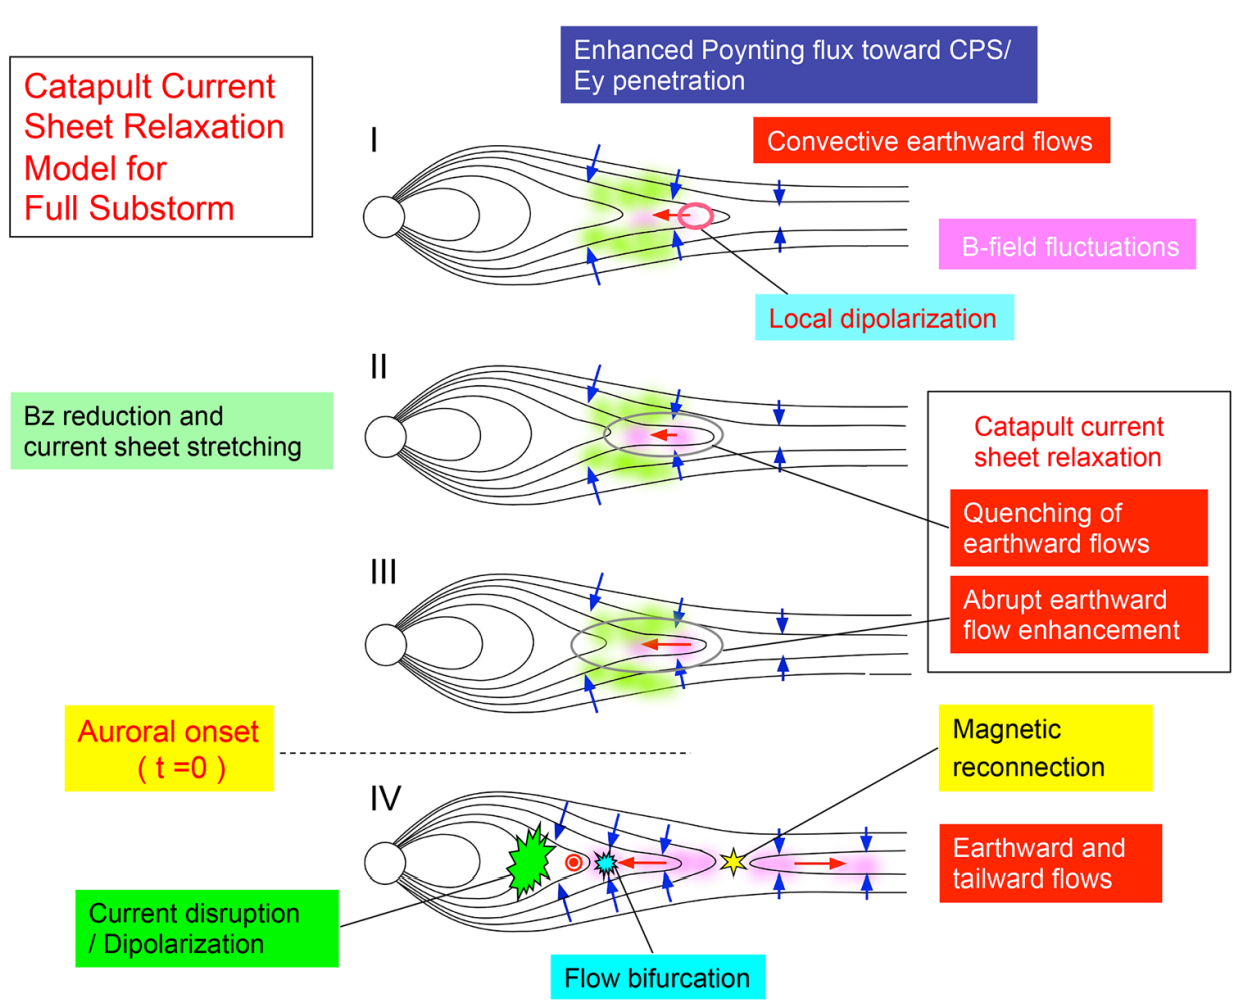
\includegraphics[width=\linewidth]{gfx/substorm-catapult}
	\caption{A substorm model based on \textit{in situ} \citep{machida2009} and optical data \citep{machida2014}.}
	\label{fig:collapse}
\end{figure}
Other important processes involved in long-term evolution of aurora due to ionospheric reconfiguration include Joule heating.
Advances in observational techniques, comparative studies and increased computational power have led to refinements in these models, and this dissertation is another contribution in the observational stack.

\FloatBarrier
\subsection{Particle Loss Mechanisms}
One outcome of the loss of charged particles from the magnetosphere is the production of aurora. 
A primary driver of the finely structured aurora is substorms \citep{fukushima1962,akasofu1964,elphin1996}.
The substorm expansion phase is thought to be driven by reconnection, which is a rapid reconfiguration of open and closed field lines due to their close encounter.
During the expansion phase, a large amount of charged particles and waves are launched toward Earth.
The magnetotail plasma on the far side of the reconnection site known as a plasmoid permanently disconnects from the magnetosphere and drifts anti-sunward from Earth into the solar system. 

Substorms create an impulsive earthward restoration of the magnetotail with some of the energy carried by the Alfvén waves discussed in section \ref{sec:alfven}. 
Quantifying the energy deposition versus ionospheric altitude of precipitating electrons is central to the data inversion of this dissertation in chapters \ref{chapter:sim} and \ref{chapter:fusion}. 
Following \citet{rees1989}, we use the laboratory results of \citet{barrett1976} valid for 300..\unit[5000]{eV} that used the apparatus in Figure~\ref{fig:BellJar} to obtain
\begin{equation}\label{eq:empiricalRange}
R_{\textrm{e}^-} = 4.30 + 53.6\phi^{1.67}_{E_i}  \quad \textrm{ kg-m$^{-2}$} 
%\marginnote{e\textsuperscript- mass distance in N$_2$}
\end{equation} %Barrett & Hays p. 748
%\fxnote{Dropping the last term brings error to $10^{-8}$ from $10^{-3}$}
%\citep{JLSrs2005}  $R_{e^-} = 4.3 + 53.6K_i^{1.67} - -0.038K_i^{-0.7} \textrm{ kg-m$^2$}$} matches within 1-e3
the electron mass distance in N$_2$. 
Figure~\ref{fig:empR} shows \eqref{eq:empiricalRange}  extrapolated to energies observed at ionospheric altitudes instead of using the more complicated first principles transport equations. %paragraph 9
\begin{figure}\centering
    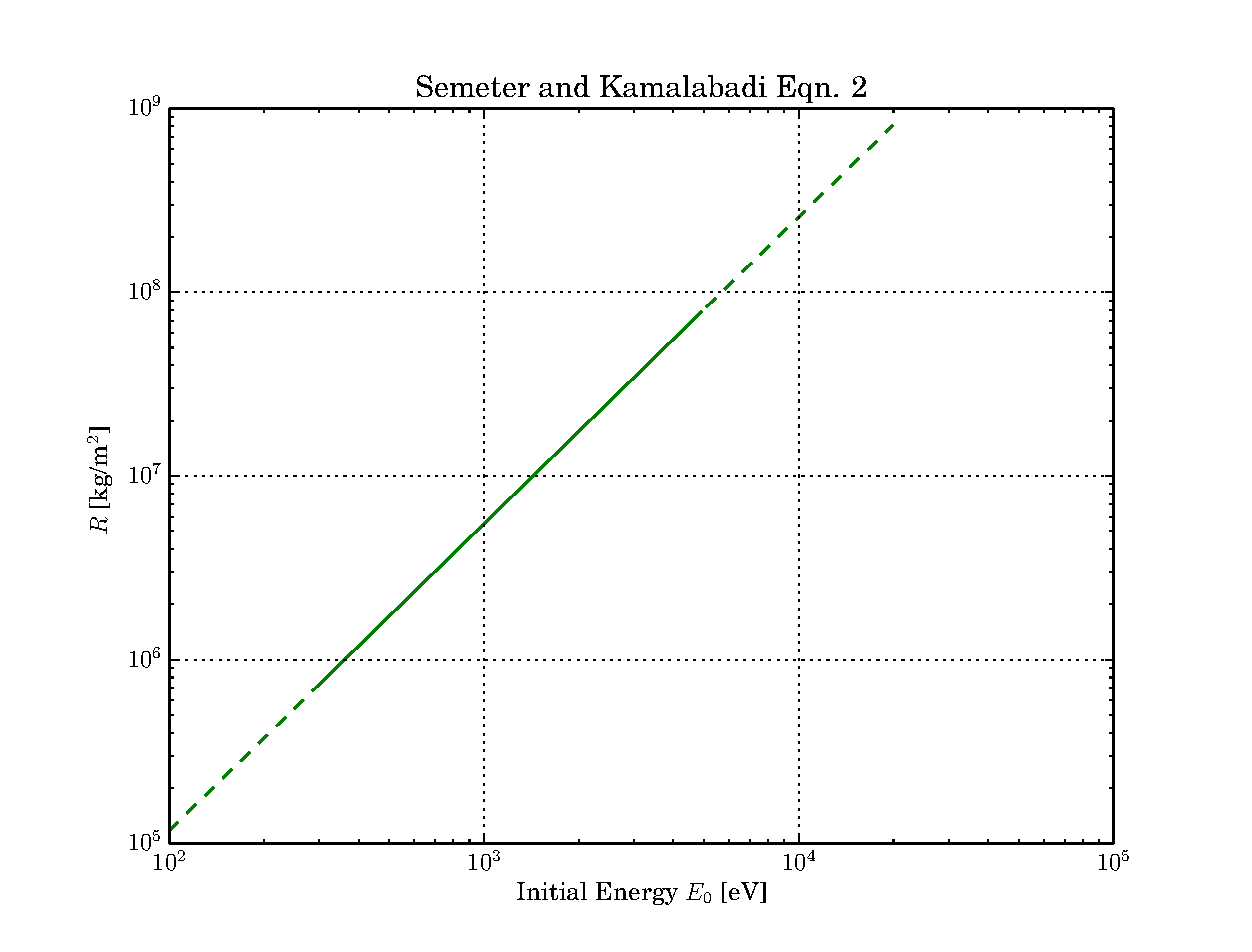
\includegraphics[width=0.8\textwidth,trim=30 10 30 20,clip]{gfx/JLSkamalabadiEqn2.eps}
    \caption{Mass-range according to \citet{semeter2005}}\label{fig:empR}
\end{figure}
The electron scattering depth for altitude $z$ is
\begin{equation}\label{eq:satm}
s_{\textrm{atm}} = \sec{\left( \theta_B \right)}\int_z^\infty \rho(z)\textrm{d}z \quad \textrm{ kg-m$^{-2}$} 
%\marginnote{e\textsuperscript- scattering depth}
\end{equation}
\citep{semeter2005}, where $\rho(z)$ is the mass density as obtained from the MSIS model. 

The maximum mass distance of the electron is $R_{\textrm{e}^-} = \pm 1$. The range $1 \leq R_{\textrm{e}^-} < 0$ accounts for backscattered electrons reflected back up toward the magnetosphere. 
An electron that travels mass distance $\Delta(s/R)$ loses $\Delta(E/\phi_{E_i})$ fraction of the initial energy. 
In the limit as $\Delta(s/R) \rightarrow 0$, the energy dissipation function
\begin{equation}\label{eq:energyDissFunc}
\Lambda = \frac{\mathrm{d}E/\phi_{E_i} }{ \mathrm{d}s/R }
\end{equation}
is defined \citep{semeter2005}. 
The energy dissipation function 
\begin{equation}\label{eq:qioniz}
q\left( z,\phi_{E_i} \right) = F \phi_{E_i} \Lambda \frac{\rho(z)}{R_{\textrm{e}^-}} \frac{1}{\Delta\varepsilon_{\textrm{ion}}}
\end{equation}
forms the core of the total ionization rate due to a precipitating electron beam \citep{rees1989}.
The average $\Delta\varepsilon_{\textrm{ion}}$ is typically taken \citep{semeter2005} to be \unit[35.5]{eV}.

We are interested in the contribution to $q$ of the differential flux $\Delta F$ impinging on the ionosphere with uniformly distributed energy range $\phi_{E_i} + \Delta\phi_{E_i}$. 
This is expressed in differential form \citep{semeter2005} 
\begin{equation}\label{eq:FredKernEner}
q\left( z,\phi_{E_i} \right) = \int_{\phi_{E_i}}^{\phi_{E_i}+\Delta\phi_{E_i}} \left[ \frac{\Lambda\rho\phi_{E_i} }{ \Delta\varepsilon_{\textrm{ion}} R } \right] \mathrm{d}\phi(E_i)d\phi
\end{equation}
where $\Delta F$ is represented by $\phi(E_i)\mathrm{d}E_i$. 
The differential system solution is aided by representing~\eqref{eq:FredKernEner} using the FIEFK
\begin{equation}\label{eq:JLSfiefk}
q(z) = \int_{E_{i,\textrm{min}}}^{E_{i,\textrm{max}}} A(z,E_i)\phi(E_i)\textrm{d}E_i
\end{equation}
where $A$ encompasses the energy deposition terms. 
The input differential number flux over all pitch angles $\phi(E_i)$ is the quantity estimated by the HiST system as described in chapter~\ref{chapter:sim}. 

%TODO $\phi$ is flux, not energy. Be sure it's consistent here.

\FloatBarrier
\subsection{Kinetic Reaction Outcomes}
A substantial fraction of the electrons precipitating from the magnetosphere into the ionosphere react kinetically with ionospheric particles in the \unit[90]{km} to \unit[500]{km} altitude range.
The electron precipitation flux incident on the top of the ionosphere as a function of energy $E$ is denoted as $\phi_{\mathrm{top}}(E)$ \citep{rees1989}.
A substantial fraction of the incident energy is reflected back to the magnetosphere according to the ionospheric albedo.
Albedo is equivalent to the reflection coefficient of a mismatched transmission line between the magnetosphere and ionosphere.
Secondary electrons produced by impact ionization in the ionosphere can reflect back into the magnetosphere.
This secondary electron population mirrors into the outer plasma with flux sufficient to heat the outer plasmasphere and hence significantly influence the conjugate ionospheric state \citep{khazanov2014}.
The kinetic reaction outcomes most relevant to ionospheric microscale features include unstable wave growth, ionospheric turbulence and the associated auroral microstructure.
An overview of the outcomes of ionospheric kinetic reactions are represented in Figure~\ref{fig:auroragen}, with a more detailed look at conditions favorable for auroral microstructure in Figure~\ref{fig:alfvenblock}.
\begin{figure}\centering
	\begin{tikzpicture}
	\node (precip) [startstop,text width=3cm] {Precipitation $\Phi_{top}(E)$ \par };
	
	\node (B) [process,below of=precip,yshift=-0.5cm] {$B_\parallel$ guided trajectory \par};
	
	\node (bang) [compute,below of=B,yshift=-0.25cm] {inelastic collision \par};
	
	\node (exc) [process,below of=bang,yshift=-0.5cm,text width=2cm] {excitation \unit[1..100]{eV} \par};
	\node (prompt)[process,below of=exc,xshift=-1.5cm,yshift=-1cm]{prompt \par};
	\node (forb)[process,right of=prompt,xshift=2cm]{forbidden \par};
	
	%\node (diss)[process,left of=exc,xshift=-2cm]{ dissociation \par};
	\node (ioni)[process,left of=exc,xshift=-3cm,text width=2cm] { impact ionization $\sim \unit[35]{eV}$ \par};
	\node (heat)[process,right of=exc,xshift=2cm] { heat \par};
	\node (radio)[startstop,right of=heat,xshift=2cm,text width=2cm]{ radio (ELF-HF) \par};
	
	\node (upflow)[startstop,below of=heat]{ion upflow \par};
	
	\node(secondary) [startstop,below of=ioni,yshift=-0.75cm,text width=2cm] {secondary electrons \par};
	
	\node (patt)[process,below of=prompt,text width=2.5cm,yshift=-0.5cm]{ atmospheric attenuation \par};
	\node (pass)[process,below of=patt,yshift=-0.5cm]{ filter: pass \par};
	
	\node (fatt)[process,below of=forb,text width=2.5cm,yshift=-0.5cm]{ atmospheric attenuation \par};
	\node (block)[process,below of=fatt,yshift=-0.5cm]{ filter: block \par};
	
	\node (chip)[startstop,below of=pass,text width=2cm,yshift=-0.25cm] {imaging chip \par};
	
	
	\draw[arrow] (precip) -- (B);
	\draw[arrow] (B) -- (bang);
	
	\draw[arrow] (bang) -- (exc);
	\draw[arrow] (bang) -- (ioni);
	%\draw[arrow] (bang) -- (diss);
	\draw[arrow] (bang) -- (heat);
	\draw[arrow] (bang) -- (radio);
	
	\draw[arrow] (ioni) --(secondary);
	
	\draw[arrow] (heat) -- (upflow);
	
	\draw[arrow] (exc) -- (prompt);
	\draw[arrow] (prompt) -- (patt);
	\draw[arrow] (patt) -- (pass);
	\draw[arrow] (pass) -- (chip);
	
	\draw[arrow] (exc) -- (forb);
	\draw[arrow] (forb) -- (fatt);
	\draw[arrow] (fatt) -- (block);
	
	\end{tikzpicture}
	\caption{Block diagram of auroral optical emissions generation and observation.
	The \texttt{filter} blocks represent emissions that are passed or blocked by HiST bandstop filtering.}
	\label{fig:auroragen}
\end{figure}


\FloatBarrier
\subsection{Radar Probing of Ionospheric Turbulence}
Two of the elementary electrostatic plasma wave modes discovered and characterized by \citet{tonks1929} \citep{hershkowitz2009} with the apparatus of Figure~\ref{fig:langmuirtube}  are the ion-acoustic wave and Langmuir (electron-acoustic) wave, with $\vect{k} \parallel \vect{B}$.
\begin{figure}
	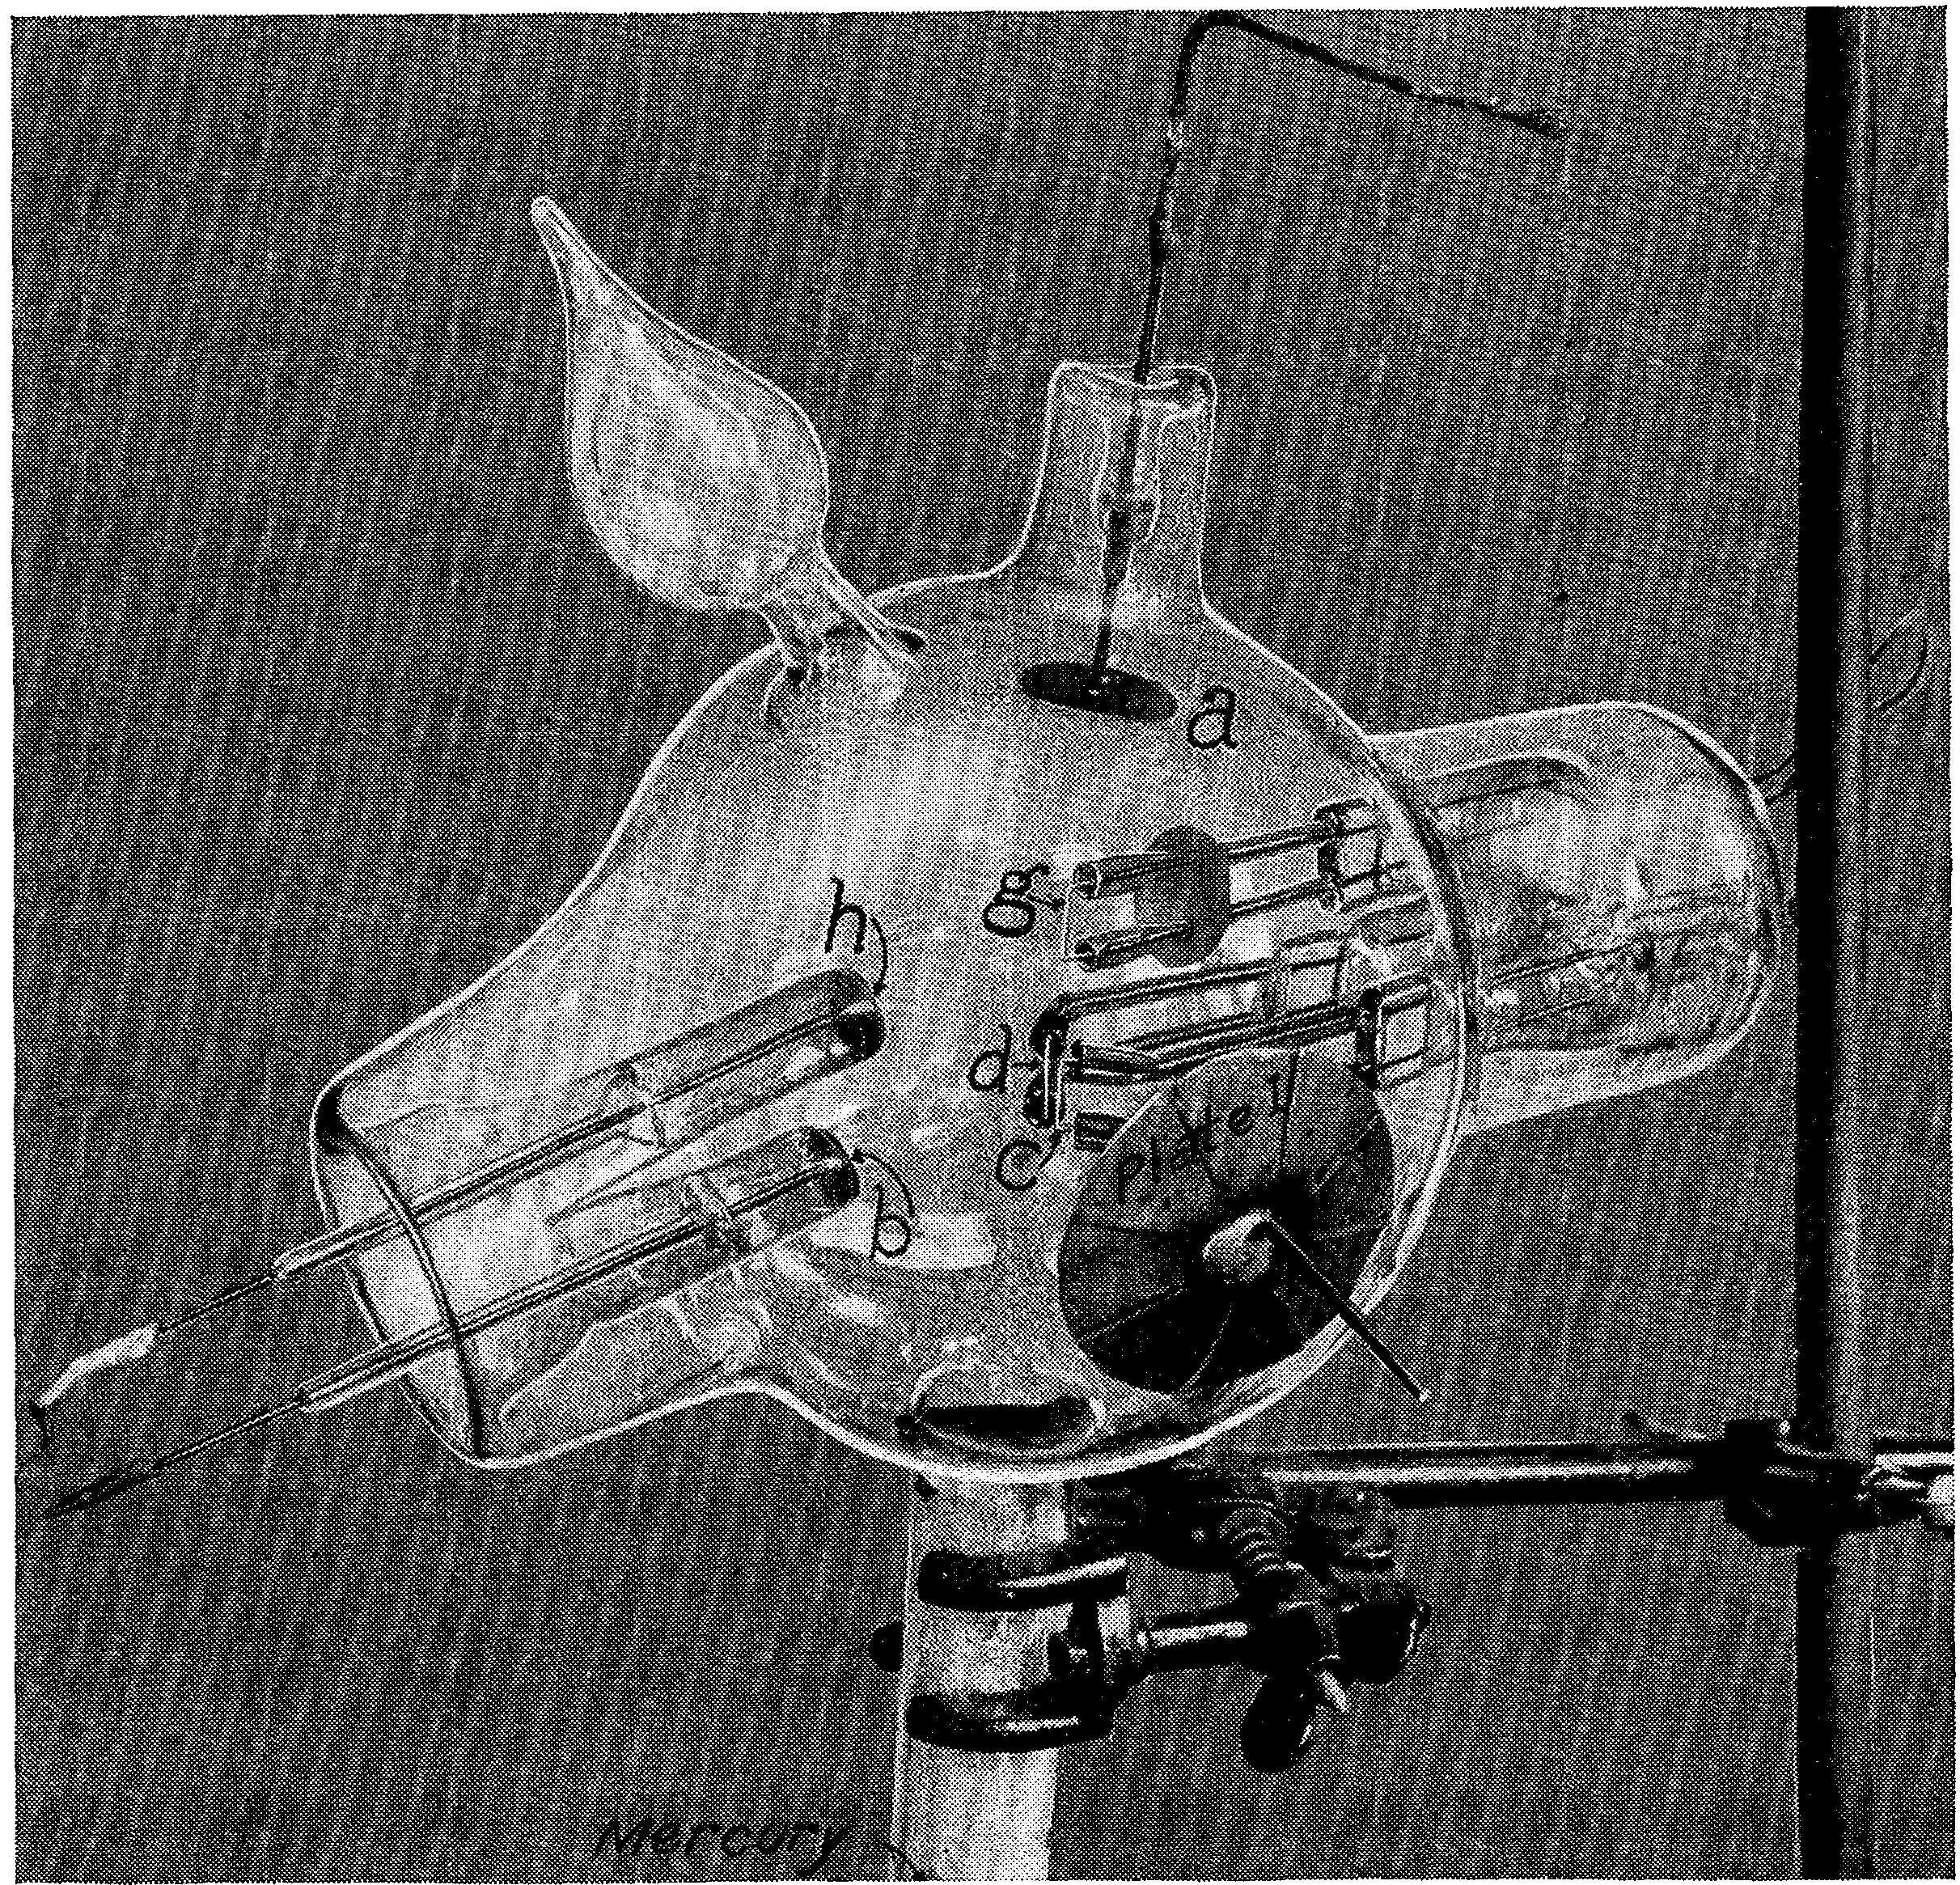
\includegraphics[width=\linewidth]{gfx/langmuir-tube}
	\caption{Apparatus used by Langmuir in \citet{tonks1929} to characterize several ion and electron plasma waves.}
	\label{fig:langmuirtube}
\end{figure}
The dispersion relation for Langmuir waves is
\begin{equation}
\omega ^{2} = \omega _{pe}^{2}+3/2 k^{2}v_{e}^{2}
\end{equation}
where electron thermal velocity 
\begin{equation}
v_e = \sqrt{2 \frac{T_0}{m_e}}
\end{equation}
and $T_0$ is the temperature of the unperturbed cold plasma background.
If we suppose that background cold plasma density $n_0$ is small or that $k_\parallel$ is small, the typical observation of ISR plasma line frequency $\omega \sim \omega_{pe}$ is realized \citep{akbaridis}.
The dispersion relation for ion-acoustic waves is
\begin{equation}
\omega ^{2} = k^{2}{\frac{k_B(T_{e} + 3 T_{i})}{m_i}}
\end{equation}
and this gives rise to the ``ion line'' as depicted in Figure~\ref{fig:isrmorph}, from which the plasma parameters $n_e, T_e, T_i, v_i$ can be estimated by ISR \citep{swobodathesis}.

Very strong radar scattering can occur at radar frequency $\omega_0 \gg \omega_{pe}$, where plasma frequency is \citep{langmuir1928,chenbook}
\begin{equation}\label{eq:wpe}
\omega_{pe} = \sqrt{\frac{n_e e^2}{\epsilon_0 m_e}}.
\end{equation}
Although phase shift is expected for $\omega > \omega_{pe}$, a fact exploited in the use of GNSS TEC measurements \citep{coster1992}, constructive reflections from a sufficiently large power aperture radar yield a detectable signal.
Other minuscule signals detectable with ISR include meteoric smoke particles \citep{mahmoudian2017,baumann2016,hsu2011} and space debris down to \unit[3]{cm} at \unit[1000]{km} range with \unit[100]{ms} integration time \citep{nicolls2015}.
Almost as soon as PFISR was turned on, naturally enhanced ion acoustic lines (NEIALs) were observed, which \citet{michell2008} in Figure~\ref{fig:firstpfisrneials} associated with bright auroral forms.
\begin{figure}
	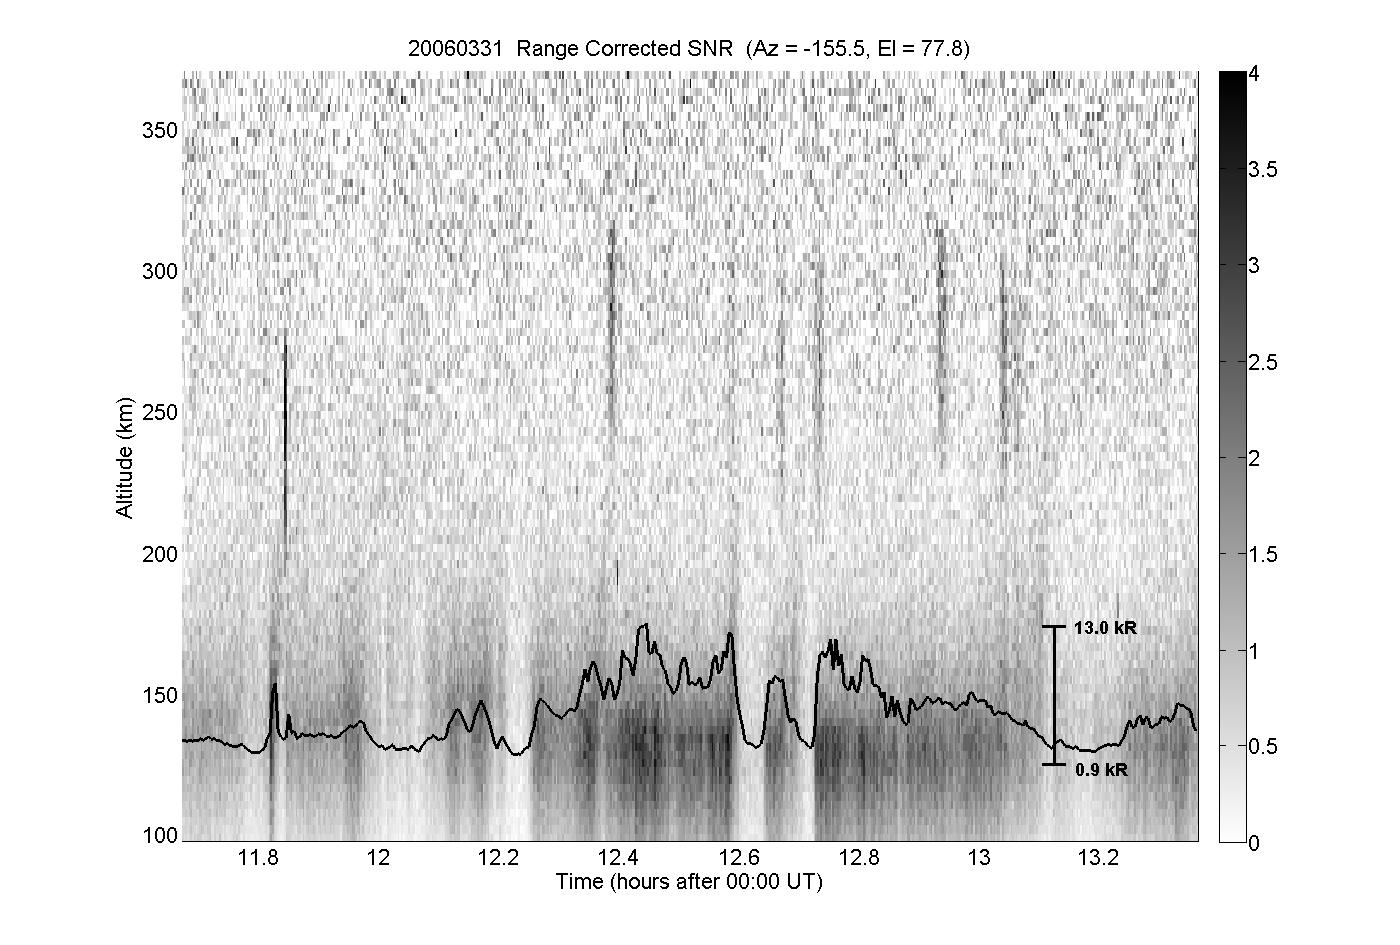
\includegraphics[width=\linewidth]{gfx/pfisrfirstneials}
	\caption{NEIALs and correlated optical intensity rise observed with the PFISR magnetic zenith beam in March 2006 \citep{michell2008}.}
	%Note, wavelength was not given in the paper. I know it's NOT the sum of all lines, but not sure which line. Probably 557.7 is my guess. Could find out from original P-DMSP data.
	\label{fig:firstpfisrneials} 
\end{figure}
NEIALs are the ISR observed results of Bragg scattering from plasma turbulence at 1/2 the radar wavenumber, leading to the ion line spectra of Figure~\ref{fig:isrmorph}(b,c).
NEIALs have been observed to occur over 140..\unit[1900]{km} altitude range \citep{schlatter2013}.





%Langmuir waves are electrostatic plasma waves where $\omega \sim \omega_{pe}$. 

%\citet{newman1994linear} notes that Langmuir bursts occur in ``moderately magnetized'' plasma where $\Omega_e \approx \omega_{pe}$.
%\citet{akbari2013} connected HF emissions in the 0.1..\unit[10]{MHz} range with NEIALS.




